% !TeX spellcheck = de_AT_frami
\section{Numerische Integration}
	\begin{enumerate}
		\item \textbf{Was bedeutet \textit{Linearität} und \textit{Positivität} des Integrals?} \\
		Eigenschaften des Integrals und der numerischen Approximation.
		\begin{itemize}
			\item Linearität: \quad \(\int_{a}^{b}\left(\alpha f(x)+\beta g(x)\right)\dif{x} = \alpha \int_{a}^{b}f(x)\dif{x}+\beta\int_{a}^{b}g(x)\dif{x}\)
			\item Positivität: \quad \(f(x)\geq0\) für alle \(x\in[a,b]\Rightarrow\int_{a}^{b}f(x)\dif{x}\geq0.\)
		\end{itemize}
		
		\item \textbf{Erklären Sie den Begriff \textit{Quadraturformel}.} \\
			Eine Quadraturformel \(Q=(b_i,c_i)^s_{i=1}\) ist eine Näherungsformel
			\begin{align*}
				I(g)=\int_{0}^{1}g(t)\dif{t}\approx\sum_{i=1}^{s}b_ig(c_i)=:Q(g)
			\end{align*}
			zur numerischen Berechnung eines Integrals auf dem Intervall \([0,1]\). Die Zahlen \(b_1,\dots,b_s\) heißen Gewichte und \(c_1,\dots,c_s\) Knoten der Quadraturformel, \(s\) ist die Anzahl der Stufen.
			Für die Knoten wird
			\begin{align*}
				0\leq c_1<c_2<\cdots<c_s\leq1
			\end{align*}
			verlangt und für die Gewichte
			\begin{align*}
				b_1+b_2+\dots+b_s=1.
			\end{align*}
			Für ein beliebiges Intervall \([a,b]\) werden die Knoten von \([0,1]\) nach \([a,b]\) transformiert und es gilt
			\begin{align*}
				I(g)=\int_{a}^{b}g(t)\dif{t}\approx(b-a)\sum_{i=1}^{s}b_i\underbrace{f(a+c_i(b-a))}_{g(c_i)}=:Q(f,[ab]).
			\end{align*}
			\begin{figure}[htbp]
				\centering
				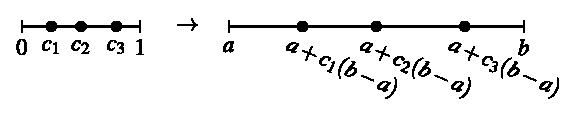
\includegraphics[width=0.4\linewidth]{kap4_1}
			\end{figure}
		
		
		\item \textbf{Nennen Sie einige einfache Quadraturformeln inklusive Knoten und Gewichte.}
			\begin{figure}[htbp]
				\centering
				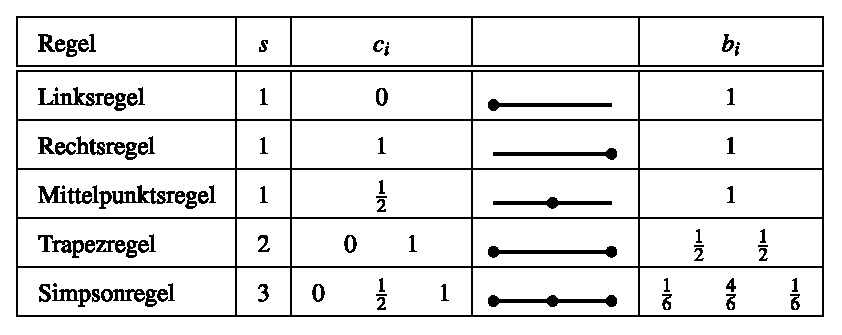
\includegraphics[width=0.6\linewidth]{kap4_2}
			\end{figure}
		
		\pagebreak
		
		\item \textbf{Erklären Sie den Begriff \textit{zusammengesetzte Quadraturformel}.} \\
			Ist der Abstand \(b-a\) sehr groß oder ändert sich der Integrand im Integrationsbereich \([a,b]\) rasch, zerlegt man \([a,b]\) in \(n\) Teilintervalle \([x_0,x_1],[x_1,x_2],\dots,[x_{n-1},x_n]\) mit \(a=x_0<x_1<x_2<\cdots<x_{n-1}<x_n=b\). Das Integral wird aufgespalten in eine Summe von \(n\) Teilintegralen über die einzelnen Teilintervalle:
			\begin{align*}
				\int_{a}^{b}f(x)\dif{x}=\int_{x_0}^{x_1}f(x)\dif{x}+\int_{x_1}^{x_2}f(x)\dif{x}+\cdots+\int_{x_{n-1}}^{x_n}f(x)\dif{x}
			\end{align*}
			Jedes dieser Teilintegrale \(\int_{x_{k-1}}^{x_k}f(x)\dif{x}\) wird mit einer Quadraturformel numerisch berechnet.\\
			Genauer Definiert mit der Definition aus 4.2: \\
			Es sei eine Quadraturformel \(Q=(b_i,c_i)^s_{i=1}\) und eine Unterteilung des Intervalls \([a,b]\) wie oben gegeben. Dann heißt eine Näherungsformel
			\begin{align*}
				\int_{a}^{b}f(x)\dif{x}\approx\sum_{k=1}^{n}Q(f,[x_{k-1}],x_k)=\sum_{k=1}^{n}h_k\sum_{i=1}^{s}b_if(x_{k-1}+c_ih_k)=:S_Q(f,x_0,\dots,x_n)
			\end{align*}
			mit \(h_k=x_k-x_{k-1}\) zusammengesetzte Quadraturformel oder Summe von Quadraturformeln. Für eine äquidistante Unterteilung von \([a,b]\) in \(n\) Teilintervalle, also
			\begin{align*}
				x_k=a+kh, \quad h=\frac{b-a}{n}, \quad k=0,\dots,n,
			\end{align*}
			haben wir folgende Näherungsformel
			\begin{align*}
				\int_{a}^{b}f(x)\dif{x}\approx h\sum_{k=1}^{n}\sum_{i=1}^{s}b_if(x_{k-1}+c_ih)=:S_Q(f,h,[a,b])=S_Q(f,h).
			\end{align*}
		
		\item \textbf{Wie erhält man Quadraturformeln mit Hilfe von Polynominterpolation?} \\
			Die zu integrierende Funktion \(g\) wird durch ein Polynom \(q\) ersetzt und dieses integriert. Die Stützstellen der Polynominterpolation sind die Knoten der Quadraturformel. Die Gewichte erhält man durch Integrieren der Lagrange-Polynome:
			\begin{align*}
				b_i=\int_{0}^{1}\ell_i(t)\dif{t},\quad \ell_i(t)=\prod_{j=1,j\neq i}^{s}\frac{t-c_j}{c_i-c_j}.
			\end{align*}
			Für die Knoten \(c_i\) gibt es verschiedene Ansätze, zum Beispiel Abgeschlossene Newton-Cotes-Formeln
			\begin{align*}
				c_i=\frac{i-1}{s-1}, \quad i=1,\dots,s.
			\end{align*}
			Für bessere Näherungen verwendet man jedoch Tschebyscheff-Knoten was zu den Clenshaw-Curtis-Formeln führt:
			\begin{align*}
				c_i=\frac{1}{2}\sin\left(\frac{2i-1}{2s}\right)+\frac{1}{2}
			\end{align*}
			
		\item \textbf{Erklären Sie den Begriff \textit{Ordnung} einer Quadraturformel. Wie bestimmt man die Ordnung?} \\
			Eine Quadraturformel \(Q=(b_i,c_i)^s_{i=1}\) hat Ordnung \(p\) genau dann, wenn alle Polynome \(q\) vom Grad \(\leq p-1\) exakt integriert werden, also \(I(q)=Q(q)\) gilt. \\
			
		
		\item \textbf{Was sind \textit{Bedingungsgleichungen}?} \\
			Alternativ muss die Quadraturformel die Bedingungsgleichung erfüllen:
				\begin{align*}
					\sum_{i=1}^{s}b_ic_i^k=\frac{1}{k+1},\quad
						k=0,\dots,p-1
				\end{align*}
		
		\item \textbf{Erklären Sie die Begriffe \textit{Fehler einer Quadraturformel} und \textit{Fehlerkonstante}.} \\
		Gegeben sei ein Intervall \([a,b]\) und die Quadraturformel \(Q(f,[a,b])=h\sum_{i=1}^{s}b_if(a+c_ih)\) mit Schrittweite \(h=b-a\). Für stetige Funktionen \(f\in\mathscr{C}([a,b])\) definiert man den Fehler der Quadraturformel als
		\begin{align*}
			E(f)=I(f)-Q(f)=\int_{a}^{a+h}f(x)\dif{x}-h\sum_{i=1}^{s}b_if(a+c_ih).
		\end{align*}
		
		\item \textbf{Was für Abschätzungen gelten für den Fehler einer Quadraturformel bzw. einer zusammengesetzten Quadraturformel? Was muss der Integrand $f$ dabei erfüllen?} \\
			Siehe 4.5 Fehler einer Quadraturformel, Satz 4.3 Fehler einer Quadraturformel und Satz 4.4 Fehler von zusammengesetzten Quadraturformeln.
		
		\item \textbf{Was sind \textit{symmetrische Quadraturformeln} und welche Eigenschaft besitzen sie?} \\
			Eine Quadraturformel \(b_i,c_i)^s_{i=1}\) heißt symmetrisch, wenn für die Knoten und Gewichte folgendes gilt:
			\begin{align*}
				c_i=1-c_{c+1-i}, \quad \text{und} \quad b_i=b_{s+1-i}, \quad i=1,\dots,s.
			\end{align*}
			Die Knoten und Gewichte sind also an 1/2 gespiegelt. Die Ordnung einer symmetrischen Quadraturformel ist gerade.
		
		\item \textbf{Was ist eine Gaußsche Quadraturformel? Welche Ordnung besitzen sie?} \\
			Eine Quadraturformel \(b_i,c_i)^s_{i=1}\) mit \(s\) Stufen heißt Gaußsche Quadraturformel, wenn die Knoten \(c_1,\dots,c_s\) die auf das Intervall \([0,1]\) transformierte Nullstelle \(x_1,\dots,x_s\) des Legendre Polynoms \(P_s\) vom Grad \(s\) sind, also
			\begin{align*}
				c_i=\frac{1}{2}+\frac{x_i}{2}, \quad i=1,\dots,s.
			\end{align*}
			Die Gewichte \(b_i\) sind so bestimmt, dass sie die Bedingungsgleichung
			\begin{align*}
				\sum_{i=1}^{s}b_ic_i^k=\frac{1}{k+1}, \quad k=0,\dots,s-1
			\end{align*}
			erfüllen. \\
			Die Gaußsche Quadraturformel mit \(s\) Stufen besitzt die Ordnung \(p=2s\).
			
		\item \textbf{Wie groß kann die Ordnung einer Quadraturformel maximal sein?} \\
			\(p=2s\)
		
		\item \textbf{Was gilt für die Gewichte einer Gaußschen Quadraturformel?} \\
			Die Gewichte \(b_i\) sind so bestimmt, dass sie die Bedingungsgleichung
			\begin{align*}
				\sum_{i=1}^{s}b_ic_i^k=\frac{1}{k+1}, \quad k=0,\dots,s-1
			\end{align*}
			erfüllen.
		\item \textbf{Wie funktioniert eine Schrittweitensteuerung? Erklären Sie die Begriffe \textit{Fehlerkriterium} und \textit{Fehlerschätzer}.} \\
			Um Rechenzeit einzusparen will man äquidistanten Intervallen dort verfeinert, wo sich die Funktion \(f\) rasch ändert.
			Das Fehlerkriterium dient zur Entscheidung, ob ein betrachtetes Integrationsintervall \([\alpha, \beta]\), ein Teilintervall von \([a,b]\), weiter verfeinert werden muss, oder ob das Fehlerkriterium erfüllt ist. Dann wäre der Fehler \(E(f,[\alpha,\beta])\) des Ergebnisses \(Q(f,[\alpha,\beta])\) akzeptabel.
			Da man das genaue Ergebnis nicht kennt, muss man einen Fehlerschätzer verwenden um einen Wert zu erhalten den man mit der Toleranz TOL vergleichen kann.
		
		
		\item \textbf{Erklären Sie den Begriff \textit{Richardson-Extrapolation}. Wie berechnet man est und $\mathbf{Q_{extr}}$.} \\
			
		
		\item \textbf{Was passiert bei Integranden mit Singularitäten oder Singularitäten in den Ableitungen?} \\
			Reduktion der Ordnung von \(Qc^p\) zu \(Qc^q\) mit \(q<p\).
		
		\pagebreak
		\item \textbf{Wie werden Doppelintegrale auf Rechtecken numerisch berechnet?} \\
			Durch Quadraturformeln für Rechtecke. \\
			Wir verwenden auf dem Rechteck \(R=[a,b]\times[\hat{a},\hat{b}]\) in \(x\)-Richtung einen Schritt der Quadraturformel \(Q=(b_i,c_i)^s_{i=1}\) und in \(y\)-Richtung einen Schritt der Quadraturformel \(\hat{Q}=(\hat{b}_i,\hat{c}_i)^{\hat{s}}_{i=1}\):
			\begin{align*}
				\iint_Rf(x,y)\dif{F}=\int_{a}^{b}\int_{\hat{a}}^{\hat{b}}f(x,y)\dif{y}\dif{x}\approx h\sum_{i=1}^{s}b_i\int_{\hat{a}}^{\hat{b}}f(a+c_ih,y)\dif{y}\approx h\hat{h}\sum_{i=1}^{s}\sum_{j=	1}^{\hat{s}}b_i\hat{b}_jf(a+c_ih,\hat{a}+\hat{c}_j\hat{h})
			\end{align*}
			mit \(h=b-a\) und \(\hat{h}=\hat{b}-\hat{a}\). Man hat also eine Quadraturformel mit Gewichten \(b_i,\hat{b}_j\), die \(f\) in den Punkten \((a+c_ih,\hat{a}+\hat{c}_j\hat{h})\) auswertet.
			\begin{figure}[htbp]
				\centering
				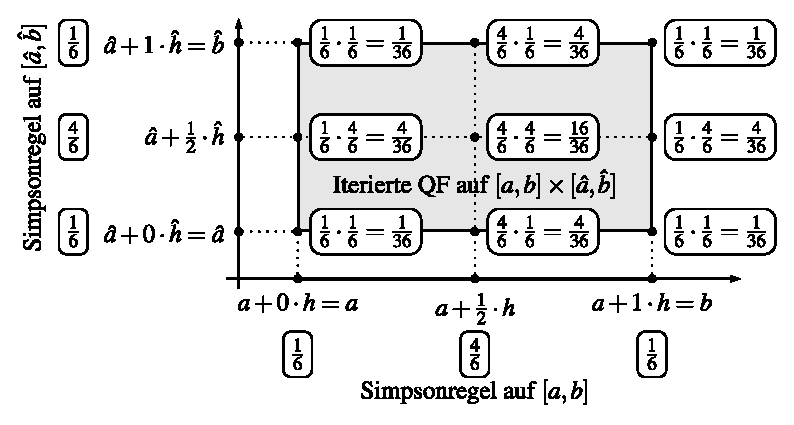
\includegraphics[width=0.7\linewidth]{kap4_3}
			\end{figure}
		
		\item \textbf{Wie werden Doppelintegrale auf Dreiecken numerisch berechnet? Wie überprüft man die Ordnung einer Quadraturformel für Dreiecke?} \\
		
		\item \textbf{Was sind \textit{baryzentrische Koordinaten}?} \\
		
	\end{enumerate}